\documentclass[Screen16to9,17pt]{foils}
\usepackage{zencurity-slides}
\externaldocument{software-security-exercises}
\selectlanguage{english}




% Secure Development Practices
% Contents

%


\begin{document}

\mytitlepage
{0. Introduction}
{Secure Development Practices}

\hlkprofiluk

\slide{Goals for today}

\hlkimage{6cm}{thomas-galler-hZ3uF1-z2Qc-unsplash.jpg}

Todays goals:
\begin{list2}
\item Welcome, what is software security and vulnerabilities
\item
\item
\item
\item
\end{list2}

  Photo by Thomas Galler on Unsplash

\slide{Software Security}

\hlkimage{10cm}{software.pdf}

\begin{list1}
\item Software security - because software is everywhere
\item Give a high level view -- don't try to remember everything just yet
\end{list1}


\slide{Contents Day 0}


\begin{list2}
\item Software security in general -- how does things fail
\item History, cases, vulnerability info etc
\item Security principles, least privilege etc.
\item Security patterns, insecure and secure design
\item Secure Development Lifecycle (SDL, SDLC, SSDL)
\item
\item Optional: Exercises, questions
\end{list2}

\slide{Contents Day 0}

\begin{list2}
\item
\item
\item
\item
\item
\item
\item Optional: Exercises, questions
\end{list2}


\slide{Current events}

Current events are always relevant, as they happen -- right NOW!
\begin{list2}
\item Fortinet CVEs - summary, make this as an exercise, evaluate a new product suggested by your boss
\item VPN -- protocols belong in network courses, but implementation is at least as important?
\item NIS2 -- impact on "software security", can you run an open source project with high risk CVEs?
\item Citrix ADC load balancers are popular in Denmark
\item CPE routes hacked and become botnet devices
\item OpenSSH even has security vulnerabilities
\end{list2}


%\slide{Current CVEs}

%We will be talking about software "problems" often named vulnerabilities, with CVE IDs
%Here are some example vulnerabilities Rezilion identified back in 2023:
%\begin{quote}
%\begin{list2}
%\item New set
%\end{list2}
%\end{quote}

%Source:\\ {\scriptsize


\slide{Microsoft Patch Tuesday: June--September 2026}

\begin{tabularx}{22cm}{|X|r| r|r|r|}\hline
Month & CVEs (Microsoft) & Critical & Zero-days & Exploited \\\hline
June  & 198--208  & 32--37 & 3 & 0 at release$^{*}$ \\\hline
July  & 569--570  & 56--59 & 3 & 2 \\\hline
August & 398--421 & 42--62 & 1--3 & 1 \\\hline
September & 964--974 & 50--113 & 2 & 2 \\\hline
\end{tabularx}

\begin{list2}
\item Vendor counts disagree by month; the ranges above reflect Microsoft's own bulletin count versus third-party trackers (Tenable, BleepingComputer, N-able, Krebs on Security, Qualys, Lansweeper)
\item Broader trackers that fold in republished third-party and Chromium-based Edge CVEs report far higher totals for the same months, e.g.\ ZDI counted 571 CVEs for June and 621 for July when Chromium fixes are included; Rapid7 counted 999 for September including 25 non-Microsoft CVEs
\item September's release is the largest in Patch Tuesday history, surpassing July; AI-assisted vulnerability discovery is cited as a factor in the increased volume
\item ZDI: 2,760 Microsoft CVEs patched so far in 2026 -- more than double any previous full year
\end{list2}

\slide{Microsoft Patch Tuesday -- June 2026}
\begin{list2}
\item 198--208 CVEs, 32--37 critical, 3 zero-days, none exploited at release
\item \emph{CVE-2026-45586} -- CTFMON EoP, public zero-day
\item \emph{CVE-2026-41089} -- Netlogon RCE CVSS 9.8, disclosed May, confirmed exploited in June
\end{list2}

\slide{Microsoft Patch Tuesday -- July 2026}
\begin{list2}
\item 569--570 CVEs, 56--59 critical, 3 zero-days, 2 exploited
\item \emph{CVE-2026-56155} -- AD FS EoP, exploited zero-day
\item \emph{CVE-2026-56164} -- SharePoint EoP, exploited zero-day
\item Largest Patch Tuesday release at the time, AI-assisted vulnerability discovery cited as a factor
\end{list2}

\slide{Microsoft Patch Tuesday -- August 2026}
\begin{list2}
\item 398--421 CVEs, 42--62 critical, 1 exploited zero-day
\item \emph{CVE-2026-68820} -- afd.sys (WinSock) EoP, CVSS 7.0, on CISA KEV\\
\link{https://www.tenable.com/blog/microsofts-august-2026-patch-tuesday-addresses-398-cves-cve-2026-68820}\\
Exercise -- check if any of these still affect your organizations
\item Vendor counts disagree by month -- Microsoft's own bulletin count vs.\ third-party trackers
\end{list2}

\slide{Microsoft Patch Tuesday -- September 2026}
\begin{list2}
\item 964--974 CVEs, 50--113 critical, 2 exploited zero-days -- largest Patch Tuesday ever
\item \emph{CVE-2026-81963} -- Windows Update Stack EoP, CVSS 7.8, on CISA KEV
\item \emph{CVE-2026-85880} -- Windows ALPC heap overflow EoP, CVSS 7.8, AppContainer sandbox escape, on CISA KEV
\item \emph{CVE-2026-69730} -- Windows DNS Server RCE, use-after-free, CVSS 9.8, unauthenticated, not exploited at release\\
\link{https://www.tenable.com/blog/microsofts-september-2026-patch-tuesday-addresses-964-cves-cve-2026-81963-cve-2026-85880}
\item Out-of-band update needed days later: the patches broke Remote Desktop Services, Hyper-V Linux VMs and USB audio
\end{list2}

\slide{Not just Microsoft}
\begin{list2}
\item Microsoft is a well-known vendor here, but far from the only vendor with high numbers
\item \emph{Linux kernel} -- 5{,}681 CVEs in 2025 (highest single year ever recorded); already 2{,}308 CVEs in H1 2026, the single highest vendor count for the period\\
\link{https://linuxiac.com/linux-tops-2026-cve-charts/}
\item \emph{Fortinet} -- 27 new CVEs disclosed in a single two-day stretch in April 2026 across FortiOS, FortiSandbox, FortiWeb and more, several critical/unauthenticated\\
\link{https://www.greenbone.net/en/blog/fortinet-rce-vulnerabilities-2026-critical-vulnerabilities-in-fortisandbox/}
\item Other vendors worth showing: \emph{Oracle} (1{,}235 CVEs in a single Critical Patch Update, July 2026), \emph{Google/Chromium} (1{,}752 CVEs H1 2026), \emph{Adobe}, \emph{Apache}
\end{list2}

\slide{Vulnerabilities by type \& year}

\hlkimage{22cm}{Vulnerabilities_by_type_year.png}

Data from \link{https://www.cvedetails.com/} but see also main link: \link{https://www.cve.org/}

\slide{OWASP Top 10:2025}
\begin{list2}
\item A01:2025 - Broken Access Control
\item A02:2025 - Security Misconfiguration
\item A03:2025 - Software Supply Chain Failures
\item A04:2025 - Cryptographic Failures
\item A05:2025 - Injection -- everything from XSS to SQL injection
\item A06:2025 - Insecure Design
\item A07:2025 - Authentication Failures
\item A08:2025 - Software or Data Integrity Failures
\item A09:2025 - Security Logging and Alerting Failures
\item A10:2025 - Mishandling of Exceptional Conditions
\end{list2}
Source: \url{https://owasp.org/Top10/2025/}

\centerline{\bf It is bad!}


\slide{OWASP Top 10: first (2003) vs latest (2025)}

\begin{center}
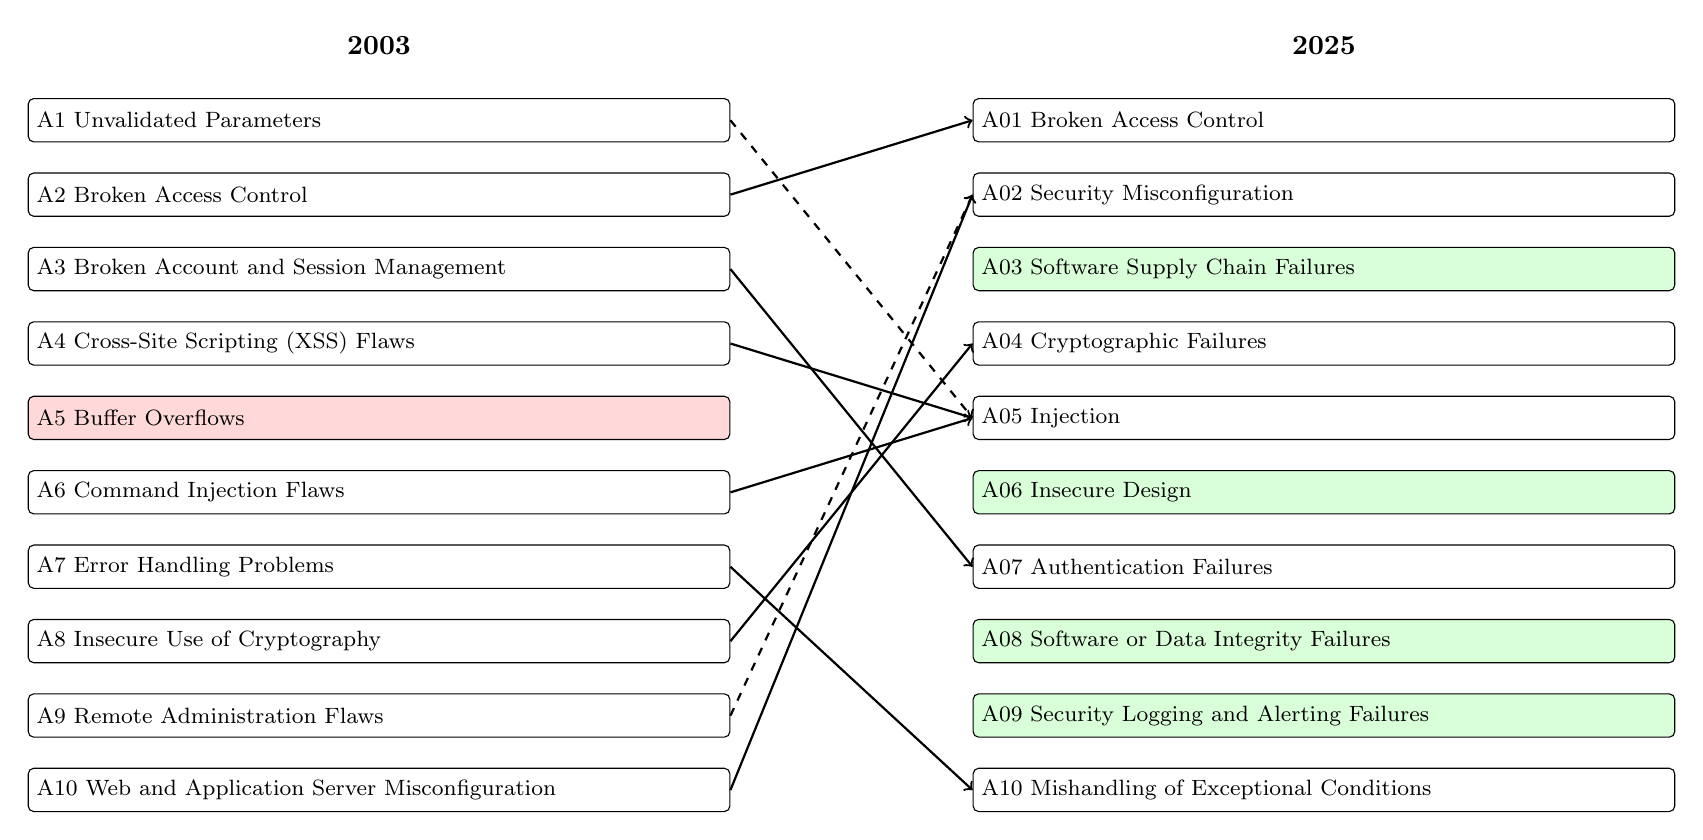
\begin{tikzpicture}[
  yscale=1.35,
  every node/.style={font=\footnotesize},
  item/.style={draw, rounded corners=2pt, text width=8.7cm, minimum height=0.55cm, inner sep=3pt},
  gone/.style={item, fill=red!15},
  new/.style={item, fill=green!15},
  map/.style={->, thick},
  loose/.style={->, thick, dashed}]

\node[font=\bfseries] at (0,0)  {2003};
\node[font=\bfseries] at (12,0) {2025};

\node[item] (o1)  at (0,-0.7) {A1 Unvalidated Parameters};
\node[item] (o2)  at (0,-1.4) {A2 Broken Access Control};
\node[item] (o3)  at (0,-2.1) {A3 Broken Account and Session Management};
\node[item] (o4)  at (0,-2.8) {A4 Cross-Site Scripting (XSS) Flaws};
\node[gone] (o5)  at (0,-3.5) {A5 Buffer Overflows};
\node[item] (o6)  at (0,-4.2) {A6 Command Injection Flaws};
\node[item] (o7)  at (0,-4.9) {A7 Error Handling Problems};
\node[item] (o8)  at (0,-5.6) {A8 Insecure Use of Cryptography};
\node[item] (o9)  at (0,-6.3) {A9 Remote Administration Flaws};
\node[item] (o10) at (0,-7.0) {A10 Web and Application Server Misconfiguration};

\node[item] (n1)  at (12,-0.7) {A01 Broken Access Control};
\node[item] (n2)  at (12,-1.4) {A02 Security Misconfiguration};
\node[new]  (n3)  at (12,-2.1) {A03 Software Supply Chain Failures};
\node[item] (n4)  at (12,-2.8) {A04 Cryptographic Failures};
\node[item] (n5)  at (12,-3.5) {A05 Injection};
\node[new]  (n6)  at (12,-4.2) {A06 Insecure Design};
\node[item] (n7)  at (12,-4.9) {A07 Authentication Failures};
\node[new]  (n8)  at (12,-5.6) {A08 Software or Data Integrity Failures};
\node[new]  (n9)  at (12,-6.3) {A09 Security Logging and Alerting Failures};
\node[item] (n10) at (12,-7.0) {A10 Mishandling of Exceptional Conditions};

\draw[loose] (o1.east)  -- (n5.west);
\draw[map]   (o2.east)  -- (n1.west);
\draw[map]   (o3.east)  -- (n7.west);
\draw[map]   (o4.east)  -- (n5.west);
\draw[map]   (o6.east)  -- (n5.west);
\draw[map]   (o7.east)  -- (n10.west);
\draw[map]   (o8.east)  -- (n4.west);
\draw[loose] (o9.east)  -- (n2.west);
\draw[map]   (o10.east) -- (n2.west);
\end{tikzpicture}
\end{center}

{\footnotesize Red: no longer on the list. Green: no 2003 counterpart. Dashed: loose mapping.
\link{https://owasp.org/Top10/2025/}}



\slide{What is Infrastructure -- Software}


\hlkimage{10cm}{alexander-schimmeck-SeeM4AnkEHE-unsplash.jpg}

\begin{list2}
\item Enterprises today have a lot of computing systems supporting the business needs
\item These are very diverse and often discrete systems
\end{list2}

\hfill Photo by Alexander Schimmeck on Unsplash

\slide{Business Challenges}

\hlkimage{7cm}{adam-bignell-9tI2z5VZIZg-unsplash.jpg}

\begin{list2}
\item Accumulation of software
\item Legacy systems
\item Partners
\item Various types of data
\item Employee churn, replacement \hfill Photo by Adam Bignell on Unsplash
\end{list2}


\slide{Software Challenges}

\hlkimage{7cm}{john-barkiple-l090uFWoPaI-unsplash.jpg}

\begin{list2}
\item Complexity
\item Various languages
\item Various programming paradigms, client server, monolith, Model View Controller
\item Conflicting data types and available structures
\item Steam train vs electric train \hfill Photo by John Barkiple on Unsplash

\end{list2}




\slide{Developers Challenges}

\hlkimage{10cm}{kelly-sikkema-YK0HPwWDJ1I-unsplash.jpg}

\begin{list2}
\item Work in teams across organisation - and partners, vendors, sub-contractors
\item Work with legacy systems, old technology
\item Learn new Technologies \hfill Photo by Kelly Sikkema on Unsplash
\end{list2}




\slide{Integration Challenges}

% hands

\hlkimage{10cm}{thomas-drouault-IBUcu_9vXJc-unsplash.jpg}

\begin{list2}
\item Enable communication between components
\item Need mediator, interpreter, translator
\item Recognize standard patterns \hfill Photo by Thomas Drouault on Unsplash
\end{list2}





\breakdance

% Lesson 1

\slide{Part 1}





\breakdance

% Lesson 2

\slide{Part 2}





\breakdance

% Lesson 3

\slide{Part 3}






\breakdance

% Lesson 4

\slide{Part 4}







\breakdance

% Lesson 5

\slide{Part 5}








\breakdance

% Lesson 6

\slide{Part 6}








\breakdance


% Lesson 7

\slide{Part 7: Optional: Exercises, questions}



\slide{Prerequisites}

\begin{list2}
\item I recommend doing exercises
\item I will use Linux and Kubernetes, but previous Linux and Unix knowledge is not needed
\item It is recommended to use containers and virtual machines for the exercises
\item Web security is a great example since the web server runs on top of operating systems and lower, plus it runs application frameworks, code by the developers etc

\item Security and most internet related security work has the following requirements:\\
Network experience, Server experience, TCP/IP principles - often in more detail than a common user, Programming is an advantage, for automating things
\end{list2}

\slide{More than half of Microsoft Azure Cloud runs Linux}

%\hlkimage{}{}

\begin{quote}
{\large Run Linux virtual machines (VMs) on Azure}

Efficiently run Linux workloads on Azure with built-in security and management

More than 60\% of customer cores in Azure run Linux workloads. Choose from popular Linux distributions including Red Hat, SUSE, Ubuntu, Debian, Flatcar, and Oracle Linux. Use preconfigured solutions from Oracle and other open-source VM-compatible providers and find Azure-optimized Linux VM images from publishers of your choice.
\end{quote}
Source: \url{https://azure.microsoft.com/en-us/products/virtual-machines/linux}


\slide{Hackerlab Setup}

\hlkimage{6cm}{hacklab-1.png}

\begin{list2}
\item Hardware: modern laptop CPU with virtualisation\\
Dont forget to enable hardware virtualisation in the BIOS
\item Virtualisation software: VMware, Virtual box, HyperV pick your poison
\item Also recommended RancherDesktop with Kubernetes as the the vulnerable systems
\item Hackersoftware: Kali Virtual Machine amd64 64-bit \link{https://www.kali.org/}
\item Linux server system: Debian amd64 64-bit \link{https://www.debian.org/}
\item Setup instructions can be found at \link{https://codeberg.org/kramse/kramse-labs}
\end{list2}



\slide{Why Kubernetes / k3s?}

\hlkimage{17cm}{kubernetes-anywhere.png}

We often use a small local Kubernetes cluster (k3s, via Rancher Desktop) as the runtime for exercises. It gives everyone the same container-based exercise environment regardless of laptop OS (Windows, Mac, Linux).

\begin{list2}
  \item Faster to start, stop, and reset an exercise than a VM
  \item Same image runs identically on your laptop as it would in production
  \item Closer to how real-world applications are actually deployed and attacked today
%  \item Lets us study Kubernetes itself as an attack surface (misconfiguration, RBAC, kube-bench, etc.)
\end{list2}

%Why k3s specifically: a lightweight, single-binary Kubernetes distribution -- easy to run locally, low resource use, same API as "full" Kubernetes.
Read more at: \link{https://k3s.io/} and \link{https://kubernetes.io/}

\slide{OWASP Juice Shop Project}

\hlkimage{3cm}{JuiceShop_Logo_100px.png}

We will also use the OWASP Juice Shop Tool Project as a running example. This is an application which is modern AND designed to have security flaws.

Read more about this project at: \link{https://www.owasp.org/index.php/OWASP_Juice_Shop_Project}\\ \link{https://github.com/bkimminich/juice-shop}

It is recommended to buy the Pwning OWASP Juice Shop Official companion guide to the OWASP Juice Shop from \link{https://leanpub.com/juice-shop} - suggested price USD 5.99



\slide{Kubernetes Security is more than just the core}

\hlkimage{12cm}{rice-container-security-1.png}
Source: \emph{Container Security}, (CS) Liz Rice, O'Reilly, Apr 2020

\begin{list2}
\item Attacks from inside, attacks inside containers
\item Some just use up resources, some attacks others, some attack the system from the inside
\item Hacking Kubernetes have a whole \emph{Chapter 3 Container Runtime Isolation}
\end{list2}


\slide{Analysis on Docker Hub malicious images}

\hlkimage{10cm}{sysdig-malicious-images.png}
This article is relevant, talking about malicious docker images\\
\link{https://sysdig.com/blog/analysis-of-supply-chain-attacks-through-public-docker-images/}



\slide{Benchmarking tools}

\begin{quote}
\faWrench\ \verb+Kube-bench+ is the industry-standard tool to automate checking Kubernetes compliance with the Center for Internet Security (CIS) Benchmark.

Kube-bench makes it easy for operators to check whether each node in their Kubernetes cluster is configured according to security best practices.
\end{quote}
Source: \link{https://info.aquasec.com/open-source}

\begin{list2}
\item CIS Kubernetes V1.24 Benchmark v1.0.0 - 09-21-2022 -- other versions exist
\item CIS Docker Benchmark v1.5.0 - 12-28-2022
\end{list2}

%\slide{Benchmarking and keeping up to date}

% Try it out \faWrench\ \verb+kube-bench+ - make some bad changes, like LKS p95 allow anonymous authentication, show why layered defense works, and how kube-bench marks it. Another example token based access, initially we have token while installing, remember to remove!
% \faWrench\ \verb+kube-hunter+ and kube-bench

\slide{Tool example kube-bench}

%\hlkimage{}{}

\begin{alltt}\scriptsize
hlk@timon:~/bin/kube-bench/kube-bench$ {\bf kubectl logs kube-bench-gdf62}
[PASS] 1.1.7 Ensure that the etcd pod specification file permissions are set to 600 or more restrictive (Automated)
[PASS] 1.1.8 Ensure that the etcd pod specification file ownership is set to root:root (Automated)
[WARN] 1.1.9 Ensure that the Container Network Interface file permissions are set to 600 or more restrictive (Manual)
[WARN] 1.1.10 Ensure that the Container Network Interface file ownership is set to root:root (Manual)
[PASS] 1.1.11 Ensure that the etcd data directory permissions are set to 700 or more restrictive (Automated)
[FAIL] 1.1.12 Ensure that the etcd data directory ownership is set to etcd:etcd (Automated)
...
== Summary policies ==
0 checks PASS
0 checks FAIL
35 checks WARN
0 checks INFO

== Summary total ==
63 checks PASS
10 checks FAIL
58 checks WARN
0 checks INFO

\end{alltt}

\begin{list2}
\item \url{https://github.com/aquasecurity/kube-bench} also check out Lynis \url{https://cisofy.com/lynis/}
\end{list2}




\slide{Kubernetes lab setup -- proof of concept}

\hlkimage{4cm}{hacklab-1.png}

\begin{list2}
\item Hardware: any modern PC with modern CPU and virtualisation\\
Don't forget to enable it in the BIOS
\item Software: your favourite operating system
\item Container software: pick your poison
\item Hacker software: maybe a nearby Kali as a Virtual Machine \link{https://www.kali.org/}
\item Smallest Kubernetes: Minikube -  I have run this on Debian
\item Production deployment probably would use better tools like \faWrench\ \verb+Kubeadm+
\end{list2}

We will run K3s in this version of the course! Recommend using the Rancher Desktop version



\slide{Optional: Exercises, questions}


\slide{A manual page}

\begin{alltt}\footnotesize
\small
NAME
     cal - displays a calendar
SYNOPSIS
     cal [-jy] [[month]  year]
DESCRIPTION
   cal displays a simple calendar.  If arguments are not specified, the cur-
   rent month is displayed.  The options are as follows:
   -j      Display julian dates (days one-based, numbered from January 1).
   -y      Display a calendar for the current year.

The Gregorian Reformation is assumed to have occurred in 1752 on the 3rd
of September.  By this time, most countries had recognized the reforma-
tion (although a few did not recognize it until the early 1900's.)  Ten
days following that date were eliminated by the reformation, so the cal-
endar for that month is a bit unusual.
\end{alltt}

\slide{The year 1752}

\begin{alltt}\footnotesize
  user@Projects:$ cal 1752
...
         April                  May                   June
  Su Mo Tu We Th Fr Sa  Su Mo Tu We Th Fr Sa  Su Mo Tu We Th Fr Sa
            1  2  3  4                  1  2      1  2  3  4  5  6
   5  6  7  8  9 10 11   3  4  5  6  7  8  9   7  8  9 10 11 12 13
  12 13 14 15 16 17 18  10 11 12 13 14 15 16  14 15 16 17 18 19 20
  19 20 21 22 23 24 25  17 18 19 20 21 22 23  21 22 23 24 25 26 27
  26 27 28 29 30        24 25 26 27 28 29 30  28 29 30
                        31
          July                 August              September
  Su Mo Tu We Th Fr Sa  Su Mo Tu We Th Fr Sa  Su Mo Tu We Th Fr Sa
            1  2  3  4                     1  {\bf        1  2 14 15 16}
   5  6  7  8  9 10 11   2  3  4  5  6  7  8  17 18 19 20 21 22 23
  12 13 14 15 16 17 18   9 10 11 12 13 14 15  24 25 26 27 28 29 30
  19 20 21 22 23 24 25  16 17 18 19 20 21 22
  26 27 28 29 30 31     23 24 25 26 27 28 29
                        30 31
...
\end{alltt}


% \demo{ex:sw-basicLinuxetc}


\demo{ex:prepare-for-course}

\demo{ex:sw-kubernetes}



\demo{ex:sw-kubebench-k3s}
\demo{ex:sw-trivy-k3s}

\demo{ex:sw-startjuice}


\end{document}
